% Task 1

\renewcommand{\taskone}{
    \newtask
    
    \begin{instructions}
        Replace $2$ by $4$ in front of $\sqrt{n}$ in the denominator of the second fraction.
    \end{instructions}
}




% Task 2

\renewcommand{\tasktwo}{
    \newtask
    
    \begin{instructions}
        Add a middle dot (``$\cdot$'') before both ``$(\Delta'-2c_1)$'' and ``$(4c_w-2c_1)$'' in the numerator of the fraction on the last line.
    \end{instructions}
}




% Task 3

\renewcommand{\taskthree}{
    \newtask
    
    \begin{instructions}
        Replace ``$h$'' by ``$h^2$'' in the denominator of the fraction between square brackets in equation (5).
    \end{instructions}
}




% Task 4

\renewcommand{\taskfour}{
    \newtask
    
    \begin{instructions}
        Sort the rows of the table by the values in the ``FWP'' column in \emph{ascending} order (minimum in the first row, maximum in the last row).
    \end{instructions}
}




% Task 5

\renewcommand{\taskfive}{
    \newtask
    
    \begin{instructions}
        Replace the values in the following cells (keep the same uncertainty):
        
        \begin{center}
            \begin{tabular}{lllr}
                \textbf{Row} & & \textbf{Column} & \textbf{New value} \\
                \midrule
                $\alpha = 1$ & $\epsilon = 0.01$ & \textsc{en}$\shortrightarrow$\textsc{ja} & $16.34$ \\
                $\alpha = 1$ & $\epsilon = 0.1$ & \textsc{de}$\shortrightarrow$\textsc{en} & $24.06$ \\
                $\alpha = 1.5$ & $\epsilon = 0.01$ & \textsc{en}$\shortrightarrow$\textsc{de} & $5.87$ \\
            \end{tabular}  
        \end{center}
    \end{instructions}
}




% Task 6

\renewcommand{\tasksix}{
    \newtask
    
    \begin{instructions}
        Remove the ``Arch'' column.
    \end{instructions}
}




% Task 7

\renewcommand{\taskseven}{
    \newtask
    
    \begin{instructions}
        % Resize both images to make their widths match the width of the coloured box they correspond to.
        Resize the image so that it has the same width than the coloured box displayed below.
    \end{instructions}
}




% Task 8

\renewcommand{\taskheight}{
    \newtask
    
    \begin{instructions}
        The image used in the \texttt{wrapfigure} environment has a lot of whitespace around its content.
        Make the necessary changes to merge the black frame within the image with the black lines above and below.
    \end{instructions}
}




% Task 9

\renewcommand{\tasknine}{
    \newtask
    
    \begin{instructions}
        Hide the second graph (the blue line chart).
    \end{instructions}
}




% Task 10

\renewcommand{\taskten}{
    \newtask
    
    \begin{instructions}
        Resize the cells of the layout such that
        \begin{itemize}
            \item both image have the same height (the horizontal black lines must be aligned);
            \item the two cells span over all the horizontal space of the row.
        \end{itemize}
    \end{instructions}
}





% Task 11

\renewcommand{\taskeleven}{
    \newtask
    
    \begin{instructions}
        Reorganise the cells to make the images form the following pattern (on three rows instead of four): \\[1ex]

        \centering
        \begin{tabular}{rcrcrcr}
            1 & ~ & 4 & ~ & 7 & ~ & 10 \\
            2 & ~ & 5 & ~ & 8 & ~ & 11 \\
            3 & ~ & 6 & ~ & 9 & ~ & 12
        \end{tabular} \\[1em]

        All the images must have the same size and there must be no overlapping.
    \end{instructions}
}





% Task 12

\renewcommand{\tasktwelve}{
    \newtask
    
    \begin{instructions}
        Make the necessary changes so that each logo of this fake front cover
        \begin{itemize}
            \item has the same width than the colored box it corresponds to;
            \item is aligned with the colored box it corresponds to.
        \end{itemize}
    \end{instructions}
    }



%%%%%%%%%%%%%%%%%%%%%%%%%%%%%%%%%%%%%%%%%%%%%%%%%%%%
%%%%%%%%%%%%%%%%%%%%   TASK 1   %%%%%%%%%%%%%%%%%%%%
%%%%%%%%%%%%%%%%%%%%%%%%%%%%%%%%%%%%%%%%%%%%%%%%%%%%

% Equation taken from https://arxiv.org/abs/2103.09279
\taskone
    
\begin{code}
%%%%%%%%%%%%%%%%%%%%%%%%%%%%%%%% START EDITING HERE
    \begin{imaths}
         \int_0^T
      h_j(t)^\mathrm{T} h_k(t)
      \mathrm{d} t
      =
      {\begin{bmatrix}
        \langle \varphi_j, \varphi_k\rangle & \langle \varphi_j, \psi_k\rangle\\
        \langle \psi_j, \varphi_j\rangle & \langle \psi_j, \psi_k\rangle
      \end{bmatrix}}
      =
      \frac{1}{2}\delta_{jk}
      I_2,
    \end{imaths}
%%%%%%%%%%%%%%%%%%%%%%%%%%%%%%%% STOP EDITING HERE
\end{code}

\newpage





%%%%%%%%%%%%%%%%%%%%%%%%%%%%%%%%%%%%%%%%%%%%%%%%%%%%
%%%%%%%%%%%%%%%%%%%%   TASK 2   %%%%%%%%%%%%%%%%%%%%
%%%%%%%%%%%%%%%%%%%%%%%%%%%%%%%%%%%%%%%%%%%%%%%%%%%%

% Equation taken from https://arxiv.org/abs/2103.09261
\tasktwo

\begin{code}
%%%%%%%%%%%%%%%%%%%%%%%%%%%%%%%% START EDITING HERE
    \begin{imaths}
       A_{z^m}^*(H_k)(z)&=\sum_{n=0}^\infty \frac{\lambda^n}{\prod_{j=0}^{n-1}(k+j(m-1))}A_{z^m}^*\left(z^{k+n(m-1)}\right)\\
       &=0+\sum_{n=1}^\infty \frac{\lambda^n}{\prod_{j=0}^{n-1}(k+j(m-1))}A_{z^m}^*\left(z^{k+n(m-1)}\right)\\
       &=\sum_{n=1}^\infty \frac{\lambda^n}{\prod_{j=0}^{n-1}(k+j(m-1))}\cdot(k+n(m-1)-m+1)\cdot\left(z^{k+n(m-1)-m+1}\right)\\
       &=\sum_{n=1}^\infty \frac{\lambda^n}{\prod_{j=0}^{n-1}(k+j(m-1))}\cdot(k+(n-1)(m-1))\cdot\left(z^{k+(n-1)(m-1)}\right)\\
        &=\sum_{n=1}^\infty \frac{\lambda\cdot\lambda^{n-1}}{\prod_{j=0}^{n-1}(k+j(m-1))}\left(z^{k+(n-1)(m-1)}\right)\\
        &=\lambda\cdot \sum_{n=0}^\infty \frac{\lambda^n}{\prod_{j=0}^{n-1}(k+j(m-1))}z^{k+n(m-1)}\\
        &=\lambda H_k(z)
    \end{imaths}
%%%%%%%%%%%%%%%%%%%%%%%%%%%%%%%% STOP EDITING HERE
\end{code}

\newpage





%%%%%%%%%%%%%%%%%%%%%%%%%%%%%%%%%%%%%%%%%%%%%%%%%%%%
%%%%%%%%%%%%%%%%%%%%   TASK 3   %%%%%%%%%%%%%%%%%%%%
%%%%%%%%%%%%%%%%%%%%%%%%%%%%%%%%%%%%%%%%%%%%%%%%%%%%

% Equation taken from https://arxiv.org/abs/2103.12163
\taskthree

\begin{code}
\flushleft
%%%%%%%%%%%%%%%%%%%%%%%%%%%%%%%% START EDITING HERE
	Consider the second-order discretized advection equation
	\begin{imaths}
		\dot{q}_n(t) = -c\left(\frac{q_{n-2}(t) - 4 q_{n-1}(t) + 3q_{n}(t)}{2h}\right).\tag{1}
	\end{imaths}
	Following the usual steps, the global relation is
	\begin{imaths}
		 e^{WT} \hat{q}(k,T) - \hat{q}(k,0) - c \left( \frac{ 4 e^{-ikh} f_{0} - e^{-2ikh} f_{0} - e^{-ikh} f_{0} }{2}\right)&= 0, \quad \text{Im}(k) \leq 0,\tag{2}
	\end{imaths}
	with dispersion relation
	\begin{imaths}
		W(k) = c \,\frac{e^{-2ikh} - 4 e^{-ikh} + 3}{2h},\tag{3}
	\end{imaths}
	and nontrivial symmetry
	\begin{imaths}
		\nu_1(k) = \frac{i}{h} \ln\left(4 - e^{-ikh}\right).\tag{4}
	\end{imaths}
	Solving for $\hat{q}(k,T)$ and taking the inverse transform, we obtain
	\begin{imaths}
		q_n(T) &= \frac{1}{2\pi} \int_{-\pi/h}^{\pi/h} e^{iknh} e^{-WT} \hat{q}(k,0)\,dk\tag{5} \\
		&\quad\, + \frac{c}{2\pi} \int_{-\pi/h}^{\pi/h} e^{iknh} e^{-WT} \left( \frac{ 4 e^{-ikh} f_{0} - e^{-2ikh} f_{0} - e^{-ikh} f_{-1} }{2}\right)\,dk.
	\end{imaths}
		With the given Dirichlet boundary condition, we encounter the ghost point $f_{-1}(W,T)$, which is unknown. [\dots] Instead, we return to the continuous problem, where the PDE itself gives the Neumann boundary condition from the Dirichlet condition:
	\begin{imaths}
		q_x(0,t) = \frac{-1}{c}\,q_{t}(0,t) = \frac{-1}{c}\,\frac{\partial}{\partial t} q(0,t) = \frac{-u'(t)}{c} = \frac{-v(t)}{c}, \quad v(t) = u'(t).\tag{6}
	\end{imaths}
%%%%%%%%%%%%%%%%%%%%%%%%%%%%%%%% STOP EDITING HERE
\end{code}

\newpage





%%%%%%%%%%%%%%%%%%%%%%%%%%%%%%%%%%%%%%%%%%%%%%%%%%%%
%%%%%%%%%%%%%%%%%%%%   TASK 4   %%%%%%%%%%%%%%%%%%%%
%%%%%%%%%%%%%%%%%%%%%%%%%%%%%%%%%%%%%%%%%%%%%%%%%%%%

% Table taken from https://arxiv.org/abs/2103.09563
\taskfour

\begin{code}
%%%%%%%%%%%%%%%%%%%%%%%%%%%%%%%% START EDITING HERE
	\begin{itabular}{lc}
		\hline
		Designs& ArIc(in \%)\\ 
		\hline
		$A_1,\delta_{2}$&$41.44$\\
		$A_2,A_3,\delta_{3},\delta_{4}$&$1.57$\\
		$A_4$&$0.19$\\
		$\delta_1$&$45.45$\\
		$\delta_{5a},\delta_{5b}$&$3.00$\\
		$\delta_{5c}$&$2.28$\\
		$\delta_{10a}$&$3.31$\\
		$\delta_{10b},\delta_{15a},\delta_{15b}$&$3.94$\\
		$\delta_{10c}$&$2.38$\\
		$\delta_{15c}$&$1.04$\\
		\hline
	\end{itabular}
%%%%%%%%%%%%%%%%%%%%%%%%%%%%%%%% STOP EDITING HERE
\end{code}

\newpage





%%%%%%%%%%%%%%%%%%%%%%%%%%%%%%%%%%%%%%%%%%%%%%%%%%%%
%%%%%%%%%%%%%%%%%%%%   TASK 5   %%%%%%%%%%%%%%%%%%%%
%%%%%%%%%%%%%%%%%%%%%%%%%%%%%%%%%%%%%%%%%%%%%%%%%%%%

% Table taken from https://arxiv.org/abs/2103.09273
\taskfive

\begin{code}
%%%%%%%%%%%%%%%%%%%%%%%%%%%%%%%% START EDITING HERE
    \begin{itabular}{||c|c|c|c|c|c||}
        \hline
               & IMDB-M & IMDB-B & REDDIT-B & REDDIT-5K &  REDDIT-12K \\ \hline\hline
           \textit{baseline w/o ess.} & $38.43_{\pm 0.98}$ & $65.78_{\pm 1.25}$ & $67.33_{\pm 1.55}$ & $39.30_{\pm 1.12}$ & $28.35_{\pm 1.11}$\\ 
           \textit{baseline w/ ess.} & $38.78_{\pm 0.85}$ & $66.56_{\pm 1.13}$ & $69.33_{\pm 0.75}$ & $38.45_{\pm 0.98}$ & $30.43_{\pm 0.75}$\\ \hline\hline
    
            WL & $49.33_{\pm 4.75}$ & $73.40_{\pm 4.63}$ & $81.10_{\pm 1.90}$ & $49.44_{\pm 2.36}$ & $38.18_{\pm 1.31}$ \\
           DGK & $44.5_{\pm 0.52}$ & $66.96_{\pm 0.56}$ & $78.04_{\pm 0.39}$ & $41.27_{\pm 0.18}$ & $32.22_{\pm 0.10}$\\
          PSCN & $45.23_{\pm 2.84}$ & $71.00_{\pm 2.29}$ & $86.30_{\pm 1.58}$ & $49.10_{\pm 0.70}$ & $41.32_{\pm 0.32}$\\
          WKPI & $49.5_{\pm 0.40}$ & $75.10_{\pm 1.10}$ & \textit{n/a} & $59.50_{\pm 0.60}$ & $48.40_{\pm 0.50}$\\
           AWE & $51.54_{\pm 3.61}$ & $74.45_{\pm 5.83}$ & $87.89_{\pm 2.53}$ & $54.74_{\pm 1.91}$ & $39.20_{\pm 2.0}$\\ 
        GIN-GFL & $49.70_{\pm 2.9}$ & $74.50_{\pm 4.60}$ & $90.30_{\pm 2.60}$ & $55.70_{\pm 2.90}$ & \textit{n/a}\\ 
    
           PersLay & 48.8-52.2 & 71.2-72.6 & \textit{n/a} & 55.6-56-5 & 47.7-49.1\\ 
           GLR & \textit{n/a} & \textit{n/a} & \textit{n/a} & 54.5 & 44.5 \\ \hline\hline
    
    
           P-Eucl &  $46.45_{\pm 4.03}$ & $67.54_{\pm 3.54}$ & $71.45_{\pm 2.98}$ & $43.15_{\pm 3.12}$ & $32.56_{\pm 3.68}$\\
           P-Hybrid &  $47.87_{\pm 2.03}$ & $72.48_{\pm 4.57}$ & $72.87_{\pm 1.75}$ & $46.85_{\pm 2.17}$ & $36.42_{\pm 4.08}$\\
    
           P-Poinc &  $57.31_{\pm 4.27}$ & $81.86_{\pm 4.26}$ & $79.78_{\pm 3.21}$ & $51.71_{\pm  3.01}$ & $42.16_{\pm 3.45}$ \\ \hline
    \end{itabular}
%%%%%%%%%%%%%%%%%%%%%%%%%%%%%%%% STOP EDITING HERE
\end{code}

\newpage





%%%%%%%%%%%%%%%%%%%%%%%%%%%%%%%%%%%%%%%%%%%%%%%%%%%%
%%%%%%%%%%%%%%%%%%%%   TASK 6   %%%%%%%%%%%%%%%%%%%%
%%%%%%%%%%%%%%%%%%%%%%%%%%%%%%%%%%%%%%%%%%%%%%%%%%%%

% Table taken from https://arxiv.org/abs/2103.10958
\tasksix

\begin{code}
%%%%%%%%%%%%%%%%%%%%%%%%%%%%%%%% START EDITING HERE
    \begin{itabular}{l|r|r|r}
    \hline
        Asset class $i$ & 
        $\omega_i$ & 
        $\mu_i$ & 
        $\sigma_i$ \\
    \hline
        Real Estate Germany & 5.87\% & 5.30\% & 13.00\%\\
        Real Estate Intl.\ & 4.99\% & 6.00\% & 14.00\%\\
        Equity Intl.\ Large Cap & 6.22\% & 6.50\% & 11.18\%\\
        Equity Germany\ Large Cap & 12.74\% & 5.57\% & 14.10\%\\
        Equity Intl.\ Small Cap & 4.32\% & 5.95\% & 12.72\%\\
        Emerging Markets Equities & 8.52\% & 8.00\% & 13.00\%\\
        Private Equity  & 3.51\% & 8.50\% & 18.00\%\\
        Government Debt & 19.45\% & 0.30\% & 4.00\%\\
        Corporate Debt & 14.83\% & 1.00\% & 3.60\%\\
        Infrastructure Finance & 0.50\% & 3.20\% & 5.70\%\\
        Fixed Income & 5.33\% & 0.40\% & 2.50\%\\
        Asset Backed Securities & 7.74\% & 0.30\% & 2.10\%\\
        Cash & 5.98\% & 0.00\% & 0.00\% \\ 
    \hline
    \end{itabular}
%%%%%%%%%%%%%%%%%%%%%%%%%%%%%%%% STOP EDITING HERE
\end{code}

\newpage





%%%%%%%%%%%%%%%%%%%%%%%%%%%%%%%%%%%%%%%%%%%%%%%%%%%%
%%%%%%%%%%%%%%%%%%%%   TASK 7   %%%%%%%%%%%%%%%%%%%%
%%%%%%%%%%%%%%%%%%%%%%%%%%%%%%%%%%%%%%%%%%%%%%%%%%%%

% Images taken from Wikipedia
\taskseven

\begin{code}
%%%%%%%%%%%%%%%%%%%%%%%%%%%%%%%% START EDITING HERE
    \iincludegraphics[width=\textwidth]{doc-one/img/laser-interference.jpg}
%%%%%%%%%%%%%%%%%%%%%%%%%%%%%%%% STOP EDITING HERE
\imagesizeguidesofdocone
\end{code}

\newpage







%%%%%%%%%%%%%%%%%%%%%%%%%%%%%%%%%%%%%%%%%%%%%%%%%%%%
%%%%%%%%%%%%%%%%%%%%   TASK 8   %%%%%%%%%%%%%%%%%%%%
%%%%%%%%%%%%%%%%%%%%%%%%%%%%%%%%%%%%%%%%%%%%%%%%%%%%

% Image taken from Wikipedia
\taskheight

\begin{code}
\raggedright
\begin{wrapfigure}{r}{0.4\textwidth}
%%%%%%%%%%%%%%%%%%%%%%%%%%%%%%%% START EDITING HERE
    \centering
    \iincludegraphics[width=0.4\textwidth]{doc-one/img/nuclear-fusion.png}
%%%%%%%%%%%%%%%%%%%%%%%%%%%%%%%% STOP EDITING HERE
\wrapfigguideofdocone
\end{wrapfigure}
\kant[1-2]
\end{code}

\newpage





%%%%%%%%%%%%%%%%%%%%%%%%%%%%%%%%%%%%%%%%%%%%%%%%%%%%
%%%%%%%%%%%%%%%%%%%%   TASK 9   %%%%%%%%%%%%%%%%%%%%
%%%%%%%%%%%%%%%%%%%%%%%%%%%%%%%%%%%%%%%%%%%%%%%%%%%%

% Image taken from https://matplotlib.org/stable/gallery/index.html
\tasknine

\begin{code}
%%%%%%%%%%%%%%%%%%%%%%%%%%%%%%%% START EDITING HERE
    \iincludegraphics[width=\textwidth]{doc-one/img/matplotlib-graph.png}
%%%%%%%%%%%%%%%%%%%%%%%%%%%%%%%% STOP EDITING HERE
\end{code}

\newpage






%%%%%%%%%%%%%%%%%%%%%%%%%%%%%%%%%%%%%%%%%%%%%%%%%%%%
%%%%%%%%%%%%%%%%%%%%   TASK 10   %%%%%%%%%%%%%%%%%%%
%%%%%%%%%%%%%%%%%%%%%%%%%%%%%%%%%%%%%%%%%%%%%%%%%%%%

% Images taken from https://matplotlib.org/stable/gallery/index.html
\taskten

\begin{code}
%%%%%%%%%%%%%%%%%%%%%%%%%%%%%%%% START EDITING HERE
    \begin{gridlayout}{\textwidth}{10cm}
        \begin{row}{1}
            \begin{cell}{0.5}
                \centering
                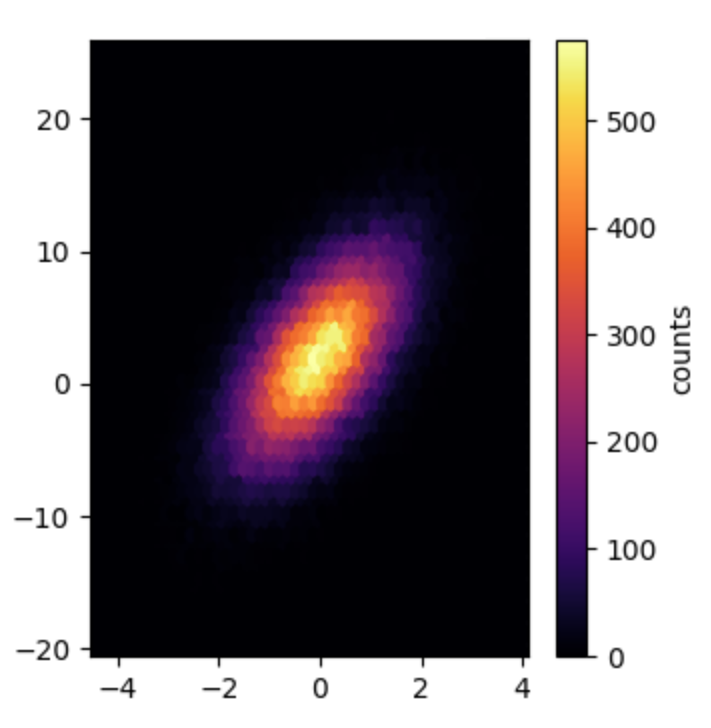
\includegraphics[width=\cellwidth]{doc-one/img/plot-1.png}
                \rule{\cellwidth}{4pt}
            \end{cell}
            \begin{cell}{0.5}
                \centering
                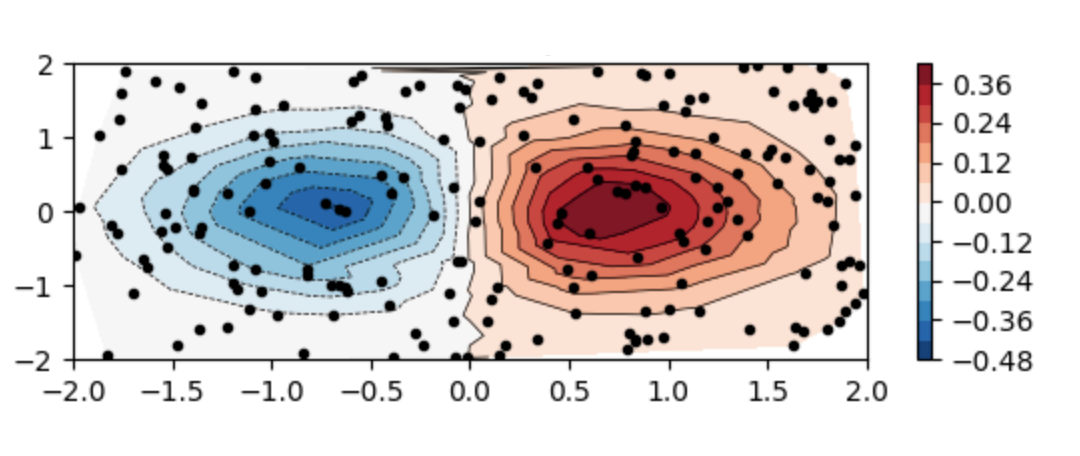
\includegraphics[width=\cellwidth]{doc-one/img/plot-2.png}
                \rule{\cellwidth}{4pt}
            \end{cell}
        \end{row}
    \end{gridlayout}
%%%%%%%%%%%%%%%%%%%%%%%%%%%%%%%% STOP EDITING HERE
\end{code}

\newpage






%%%%%%%%%%%%%%%%%%%%%%%%%%%%%%%%%%%%%%%%%%%%%%%%%%%%
%%%%%%%%%%%%%%%%%%%%   TASK 11   %%%%%%%%%%%%%%%%%%%
%%%%%%%%%%%%%%%%%%%%%%%%%%%%%%%%%%%%%%%%%%%%%%%%%%%%

% Images taken from https://arxiv.org/abs/2103.10428
\taskeleven

\begin{code}
%%%%%%%%%%%%%%%%%%%%%%%%%%%%%%%% START EDITING HERE
    \begin{gridlayout}{\textwidth}{12cm}
        \begin{row}{0.33}
            \begin{cell}{0.25}
                \centering
                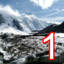
\includegraphics[width=0.9\cellwidth]{doc-one/img/thumbnail-1.png}
            \end{cell}
            \begin{cell}{0.25}
                \centering
                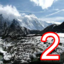
\includegraphics[width=0.9\cellwidth]{doc-one/img/thumbnail-2.png}
            \end{cell}
            \begin{cell}{0.25}
                \centering
                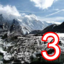
\includegraphics[width=0.9\cellwidth]{doc-one/img/thumbnail-3.png}
            \end{cell}
            \begin{cell}{0.25}
                \centering
                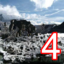
\includegraphics[width=0.9\cellwidth]{doc-one/img/thumbnail-4.png}
            \end{cell}
        \end{row}
        \begin{row}{0.33}
            \begin{cell}{0.25}
                \centering
                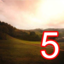
\includegraphics[width=0.9\cellwidth]{doc-one/img/thumbnail-5.png}
            \end{cell}
            \begin{cell}{0.25}
                \centering
                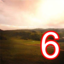
\includegraphics[width=0.9\cellwidth]{doc-one/img/thumbnail-6.png}
            \end{cell}
            \begin{cell}{0.25}
                \centering
                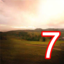
\includegraphics[width=0.9\cellwidth]{doc-one/img/thumbnail-7.png}
            \end{cell}
            \begin{cell}{0.25}
                \centering
                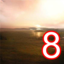
\includegraphics[width=0.9\cellwidth]{doc-one/img/thumbnail-8.png}
            \end{cell}
        \end{row}
        \begin{row}{0.34}
            \begin{cell}{0.25}
                \centering
                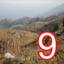
\includegraphics[width=0.9\cellwidth]{doc-one/img/thumbnail-9.png}
            \end{cell}
            \begin{cell}{0.25}
                \centering
                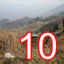
\includegraphics[width=0.9\cellwidth]{doc-one/img/thumbnail-10.png}
            \end{cell}
            \begin{cell}{0.25}
                \centering
                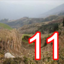
\includegraphics[width=0.9\cellwidth]{doc-one/img/thumbnail-11.png}
            \end{cell}
            \begin{cell}{0.25}
                \centering
                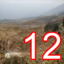
\includegraphics[width=0.9\cellwidth]{doc-one/img/thumbnail-12.png}
            \end{cell}
        \end{row}
    \end{gridlayout}
%%%%%%%%%%%%%%%%%%%%%%%%%%%%%%%% STOP EDITING HERE
\end{code}

\newpage






%%%%%%%%%%%%%%%%%%%%%%%%%%%%%%%%%%%%%%%%%%%%%%%%%%%%
%%%%%%%%%%%%%%%%%%%%   TASK 12   %%%%%%%%%%%%%%%%%%%
%%%%%%%%%%%%%%%%%%%%%%%%%%%%%%%%%%%%%%%%%%%%%%%%%%%%

\tasktwelve

\begin{code}
%%%%%%%%%%%%%%%%%%%%%%%%%%%%%%%% START EDITING HERE
    \begin{gridlayout}{\textwidth}{15cm}
        \begin{row}{0.1}
            \begin{cell}{1}
                \centering
                Internship report
            \end{cell}
        \end{row}
        \begin{row}{0.1}
            \begin{cell}{1}
                % Separator
            \end{cell}
        \end{row}
        \begin{row}{0.1}
            \begin{cell}{1}
                \centering
                \rule{0.6\cellwidth}{0.4pt}\\[1.5ex]
                {\Large Internship title}\\
                \rule{0.6\cellwidth}{0.4pt}
            \end{cell}
        \end{row}
        \begin{row}{0.45}
            \begin{cell}{1}
                % Separator
            \end{cell}
        \end{row}
        \begin{row}{0.25}
            \begin{cell}{0.5}
                \centering
                
\includegraphics[width=\cellwidth]{doc-one/img/logo-ex-situ.png}
            \end{cell}
            \begin{cell}{0.5}
                \centering
                
\includegraphics[width=\cellwidth]{doc-one/img/logo-univ-ps.png}
            \end{cell}
        \end{row}
    \end{gridlayout}
%%%%%%%%%%%%%%%%%%%%%%%%%%%%%%%% STOP EDITING HERE
\logoguidesofdocone
\end{code}

\newpage
